% Emacs, this is -*-latex-*-

% Joining the Team

\label{sec:joining}

After connecting with a splitter, incoming peers request (using a
reliable communication) to the splitter the current list of peers in
the team. To minimize the \gls{joining-time}, the peer sends a short
$[\mathtt{hello}]$ message to each other peer of the team, in parallel
with the reception of the list. When a peer of the team receives a
$[\mathtt{hello}]$, it adds the sender of the message to the team
list\footnote{Peers also updates their team list every time a chunk is
  received from a peer, incorporating the sender and the origin of the
  chunk.} and to a jagged array of peers called $\mathtt{forward}[]$
\note{(see
  \href{https://github.com/P2PSP/simulator/blob/f0c73be1817e7d3b816cc61cd2c8e59b17f9a0e6/src/core/peer_dbs.py\#L491}{$\text{forward[]}$
    in \texttt{peer.py}})}. If a peer $P_i$ has an entry
$\mathtt{forward}[P_j]=\{P_k\}$, then each chunk received by $P_i$ and
originated at $P_j$ will be forwarded to $P_k$. When an incoming peer
$P_i$ has received the list of peers, its forwarding table has been
initialized to $\mathtt{forward}[P_i]=\{\text{team}\setminus
P_i\}$. Notice that, as long as the forwarding table contains this
information, all the chunks received from the splitter will be forwarded
to the rest of the team, directly (in one single hop). So, in absence
of communication constraints, the team will be organized as a
full-connected overlay (see Fig.~\ref{fig:full_mesh}).
%
% A ver si alguno es capaz de aumentar los subcaptions!
\begin{figure*}[h!]
  \centering
  \resizebox{1.0\textwidth}{!}{
    \subfloat[A full-connected overlay.]{\label{fig:full_mesh}
      \vbox{\myfig{graphics/full-mesh}{0.9\textwidth}{400}}}
    \quad
    \subfloat[A star-shaped overlay.]{\label{fig:star}
      \vbox{\myfig{graphics/star}{0.9\textwidth}{400}}}
  }
  \caption{In a full-connected DBS team (see Subfig. (a)), all peers
    receive and send the same number of chunks. In a star-shaped DBS
    team (Subfig. (b)), $P_1$ should send all the chunks of the stream
    to the rest of the team, except those that the splitter has sent
    directly to them.}
  \label{fig:connections}  
\end{figure*}
%
\begin{figure*}[h!]
  \centering
  \begin{tabular}{cc}
    \subfloat[A full-connected overlay.]{\label{fig:full_mesh}
      \vbox{\myfig{graphics/full-mesh}{0.4\textwidth}{400}}}
    }
    &
    \resizebox{0.4\textwidth}{!}{
    \subfloat[A star-shaped overlay.]{\label{fig:star}
      \vbox{\myfig{graphics/star}{0.4\textwidth}{400}}}
    }
    \end{tabular}
  }
  \caption{In a full-connected DBS team (see Subfig. (a)), all peers
    receive and send the same number of chunks. In a star-shaped DBS
    team (Subfig. (b)), $P_1$ should send all the chunks of the stream
    to the rest of the team, except those that the splitter has sent
    directly to them.}
  \label{fig:connections}  
\end{figure*}
%

%), initializes
%the table $\mathrm{debt}[]$ (which stores the chunk debts between
%neighbor peers), and (3) sets the variable $\mathrm{neighbor}$ with an
%index to $\mathrm{forward}[]$ (see
%Sec.~\ref{sec:chunk_DBS_processing}).

The splitter, in an infinite loop: (1) listens to the incoming peers,
(2) sends to them the list of peers of the team, (3) includes the
incoming peer to the list, and (4) send a chunk to each peer in its
list. Notice that only those peers that are in the list of peers of
the splitter are considered to be in the team served by such splitter.

\begin{comment}
\begin{figure*}
  %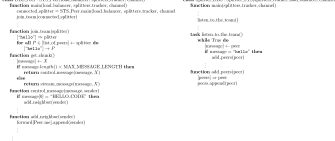
\includegraphics[width=\textwidth]{joining}
  \fig{1000}{10cm}{joining} \caption{Code related to team
    joining.\label{fig:joining}}
\end{figure*}

The new pseudo-code related to joining a team is describen in the
Fig.~\ref{fig:joining}.
\end{comment}

\begin{notex}
  See \href{https://github.com/P2PSP/simulator/blob/f0c73be1817e7d3b816cc61cd2c8e59b17f9a0e6/src/core/splitter_dbs.py#L296}{$\text{destination\_of\_chunk}[]$ in \texttt{peer\_dbs.py}}.
\end{notex}
